As mentioned in the main text, \acl{AR} is the process by which an electron is reflected as a hole at the interface between a normal-metal / superconductor interface. By modeling and fitting our data to this model we are able to extract useful quantities such as the superconducting gap size (at a specific temperature), the transparency of the interface, and the thermal broadening of our spectra from our junction size. Thus, here I layout a condensed version of the \ac{BTK} calculation for differential conductance across a normal-metal / superconducting interface then I go through pseudo-code on how to fit this calculation to our data.

\section{BTK Theory}
In 1964, Alexander F. Andreev published a paper describing a process by which an electron incident upon a superconductor forms a cooper pair in the superconductor and retro-reflects a hole\cite{Andreev1964}. This phenomena was originally used to describe the thermal conductivity properties observed in superconductors in the intermediate state where there are many normal sections in direct contact with superconducting sections. It wasn't until 1982 that Blonder, Tinkham, and Klapwijk gave a complete discussion of the phenomena including the effect of the barrier magnitude, a model for the excess current, and predictions for the differential conductance of such a junctions\cite{BTK}.\par

\subsection{The BdG Formalism}
The key innovation in the \ac{BTK} model is the use of the \ac{BdG} equations to match the wavefunctions of the quasi-particles excitations at the interface\cite{BTK}. Here I will closely follow the explanation of the \ac{BdG} equations shown in Chapter 14 of "Topological Insulators and Topological Superconductivity" by Bernevig and Hughes\cite{bernevig_hughes_2013}. First we start with the Hamiltonian for a single-particle in a simple metal.
\begin{align}
    H = \left(\frac{p^{2}}{2m}-\mu\right)I_{2\times2}
\end{align}
Where $\mu$ is the chemical potential and $I_{2\times2}$ is the identity matrix in the spin variables. The second-quantized Hamiltonian is given by:
\begin{align}
    H = \sum_{\textbf{p},\sigma}c_{\textbf{p}\sigma}^{\dagger}\left(\frac{p^{2}}{2m}-\mu\right)c_{\textbf{p},\sigma}
\end{align}
Where $c^{\dagger}$ and $c$ are the quasi-particles creation and annihilation operators respectively. Using the anti-commutativity relation of fermions, $\{c_{\textbf{p}\sigma}^{\dagger},c_{\textbf{p}'\sigma'}\}=\delta_{\sigma\sigma'}\delta_{\textbf{p}\textbf{p}'}$, we can rewrite the Hamiltonian above as,
\begin{align}
    H = \frac{1}{2}\sum_{\textbf{p}\sigma}\left[c_{\textbf{p}\sigma}^{\dagger}\epsilon(p)c_{\textbf{p}\sigma}-c_{-\textbf{p}\sigma}\epsilon(-p)c_{-\textbf{p}\sigma}^{\dagger}\right]+\frac{1}{2}\sum_{p}\epsilon(p)
\end{align}
Where $\epsilon(p)\equiv\left(\frac{p^{2}}{2m}-\mu\right)$ and we have relabeled the sum index \textbf{p} in the second term to -\textbf{p}. Here we introduce a new spinor to explicitly label the energy eigenvalues for both spins of both $\epsilon_{p}$ and $\epsilon_{-p}$. E.g., we define $\Psi_{\textbf{p}}\equiv\left(c_{\textbf{p}\uparrow} c_{\textbf{p}\downarrow} c_{-\textbf{p}\uparrow}^{\dagger}c_{-\textbf{p}\downarrow}^{\dagger}\right)$, then we can rewrite the above Hamiltonian as,
\begin{align}
    H &= \sum_{\textbf{p}}\Psi_{\textbf{p}}^{\dagger}H_{BdG}(\textbf{p})\Psi_{\textbf{p}}+\text{constant}\\
    H_{BdG}(\textbf{p}) &= \frac{1}{2}
    \begin{pmatrix}
    \epsilon(p) & 0 & 0 & 0\\
    0 & \epsilon(p) & 0 & 0\\
    0 & 0 & -\epsilon(-p) & 0\\
    0 & 0 & 0 & -\epsilon(-p)
    \end{pmatrix}
\end{align}
The point of this formalism becomes immediately apparent when we introduce a superconducting pairing potential.
\begin{align}
    H_{\Delta} &= \Delta c_{\textbf{p}\uparrow}^{\dagger}c_{-\textbf{p}\downarrow}^{\dagger}+\Delta^{*}c_{-\textbf{p}\downarrow}c_{\textbf{p}\uparrow}\\
    &= \frac{1}{2}\left[\Delta\left(c_{\textbf{p}\uparrow}^{\dagger}c_{-\textbf{p}\downarrow}^{\dagger}-c_{-\textbf{p}\downarrow}^{\dagger}c_{\textbf{p}\uparrow}^{\dagger}\right)+\Delta^{*}\left(c_{-\textbf{p}\downarrow}c_{\textbf{p}\uparrow}-c_{\textbf{p}\uparrow}c_{-\textbf{p}\downarrow}\right)\right]\\
    \therefore H+H_{\Delta} &= \sum_{\textbf{p}}\Psi_{\textbf{p}}^{\dagger}H_{BdG}(\textbf{p},\Delta)\Psi_{\textbf{p}}\\
    H_{BdG}(\textbf{p},\Delta) &= \frac{1}{2}
    \begin{pmatrix}
    \epsilon(p) & 0 & 0 & \Delta\\
    0 & \epsilon(p) & -\Delta & 0\\
    0 & -\Delta^{*} & -\epsilon(-p) & 0\\
    \Delta^{*} & 0 & 0 & -\epsilon(-p)
    \end{pmatrix}
\end{align}
Using this formalism, we can see that the pairing potential simply couples the upper and lower blocks of the $H_{BdG}$ for the simple metal Hamiltonian. From here we can diagonalize $H_{BdG}$ to obtain the energy eigenvalues.
\begin{align}
    E_{\pm} = \pm\sqrt{\epsilon(\textbf{p})^{2}+|\Delta|^{2}}
\end{align}
The quasi-particles dispersion relations for the normal metal $(|\Delta|=0)$ and the superconductor $(|\Delta|=0.1m)$ are plotted in Fig \ref{fig:AndreevDiagram} which also conveniently serves as a perfect starting point for the discussion of the \ac{BTK} calculation.\par

\begin{figure}
    \centering
    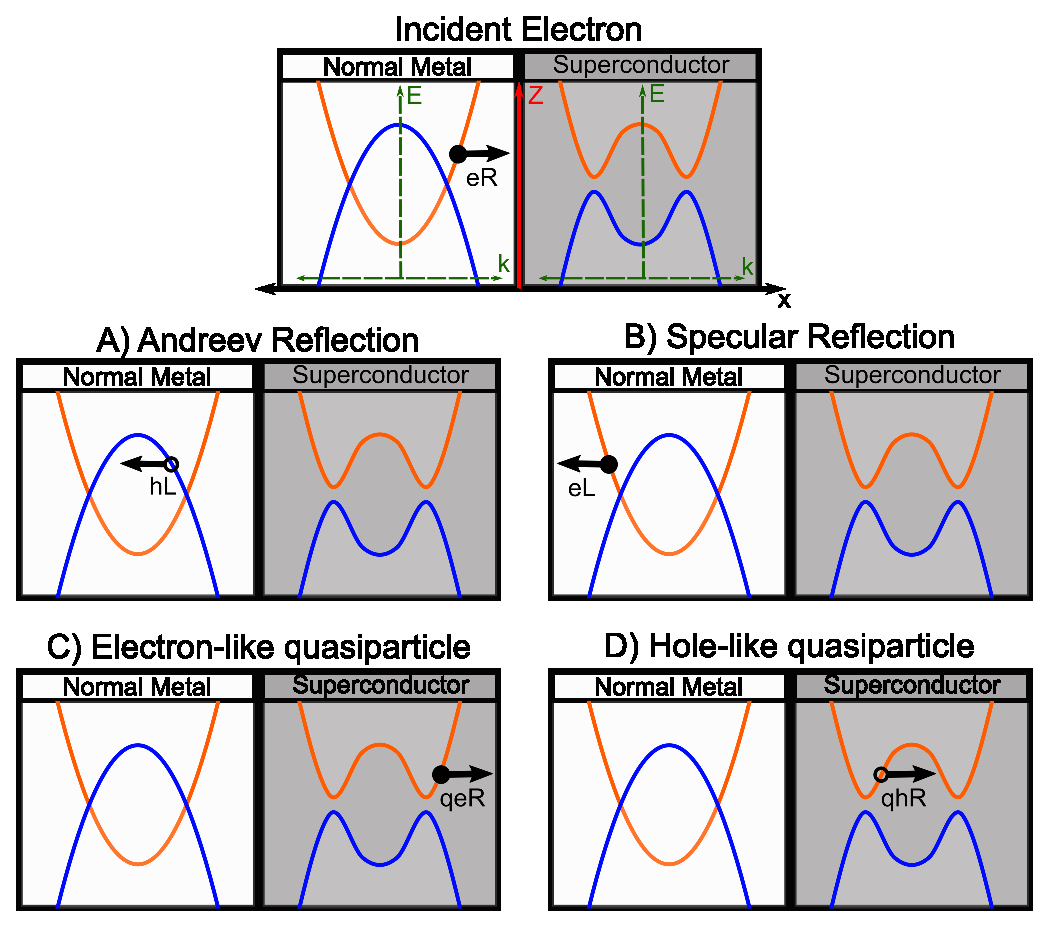
\includegraphics[width=\textwidth]{Appendices/Figures/AndreevDiagram.eps}
    \caption{Dispersion relations for a normal metal and superconductor in physical contact with one another. The red axis denotes the real-space position of the two materials with a potential barrier at their interface. The subset green, dashed axes denote the dispersion relations within the respective materials. A right-moving incident electron (top) can take one of four paths once it hits the NM/SC barrier: A) Andreev reflect as a left-moving hole, B) Normally reflect as a left-moving electron, C) Transmit as a right-moving electron-like quasi-particles, or D) Transmit as a right-moving hole-like quasi-particles.}
    \label{fig:AndreevDiagram}
\end{figure}

\subsection{The \ac{BTK} calculation}
First, we consider a normal metal in contact with a superconductor. The dispersion relations for the two are as calculated in the previous section and the barrier in the interface is modeled by a Dirac-delta function with magnitude $Z$. \ac{BTK} considers a plane-wave electron incident from the normal metal on the left side of the junction thus when the electron encounters the barrier there are four possibilities (shown in Fig \ref{fig:AndreevDiagram}):\\
\\
A) The electron is Andreev reflected as a left-moving hole and a right-moving Cooper-Pair transmits into the superconducting fluid.\\
B) The electron is specularly reflected as a left-moving electron.\\
C) The electron is transmitted as a right-moving electron-like quasiparticle.\\
D) The electron is transmitted as a right-moving hole-like quasiparticle.\\
\\
To solve for the probabilities of each process occurring we first define the momenta in the normal metal and superconductor respectively as,
\begin{align}
    k^{\pm} &= \sqrt{\frac{2m_N}{\hbar^{2}}}\sqrt{E_{FN}\pm E}\\
    q^{\pm} &= \sqrt{\frac{2m_{SC}}{\hbar^{2}}}\sqrt{E_{FSC}\pm\sqrt{E^{2}-\Delta^{2}}}
\end{align}
Then we simply match the boundary conditions, i.e., the wavefunctions and their derivatives are the same at the boundary. Starting with the wavefunctions,
\begin{align}
    \begin{pmatrix}1\\0\end{pmatrix}e^{ik^{+}x_{0}}
    + C\begin{pmatrix}1\\0\end{pmatrix}e^{-ik^{+}x_{0}}
    + D\begin{pmatrix}0\\1\end{pmatrix}e^{ik^{-}x_{0}}
    =
    A\begin{pmatrix}u_{0}\\v_{0}\end{pmatrix}e^{iq^{+}x_{0}}
    + B\begin{pmatrix}u_{0}\\v_{0}\end{pmatrix}e^{-iq^{-}x_{0}}
\end{align}
then the derivatives.
\begin{align}
    &\frac{\hbar^{2}}{2m_{N}}\left\{
    ik^{+}\begin{pmatrix}1\\0\end{pmatrix}e^{ik^{+}x_{0}}
    -ik^{+}C\begin{pmatrix}1\\0\end{pmatrix}e^{-ik^{+}x_{0}}
    +ik^{-}D\begin{pmatrix}1\\0\end{pmatrix}e^{ik^{-}x_{0}}
    \right\}\\
    &= \frac{\hbar^{2}}{2m_{SC}}\left\{
    iq^{+}A\begin{pmatrix}u_{0}\\v_{0}\end{pmatrix}e^{iq^{+}x_{0}}
    -iq^{-}B\begin{pmatrix}u_{0}\\v_{0}\end{pmatrix}e^{-iq^{-}x_{0}}
    \right\}\\
    &\qquad+H*\left\{
    A\begin{pmatrix}u_{0}\\v_{0}\end{pmatrix}e^{iq^{+}x_{0}}
    +B\begin{pmatrix}u_{0}\\v_{0}\end{pmatrix}e^{-iq^{-}x_{0}}
    \right\}
\end{align}
where $x_{0}$ is the position of the barrier (it is typically set to zero) and $u_{0}$, $v_{0}$ are the electron-weight and hole-weight of the quasiparticles, respectively. Thus the transmission coefficients are given by:
\begin{align}
    \begin{matrix}
    a=\left(\left|A\right|^{2}*\left(u_{0}^{2}-v_{0}^{2}\right)\right)\frac{q_{SC}^{+}}{k_{N}^{+}} & b=\left|B\right|^{2}*\left(u_{0}^{2}-v_{0}^{2}\right)\frac{q_{SC}}{k_{N}^{+}}\\
    c = \left|C\right|^{2} & d = \left|D\right|^{2}*\frac{k_{N}^{-}}{k_{N}^{+}}
    \end{matrix}
\end{align}

Before plugging in the momentum values there are some quick simplification we can make here to improve readability. Using, $v_{F}^{SC}=\hbar k_{FSC}/m_{SC}$ and $v_{FN}=\hbar k_{FN}/m_{N}$, we define $Z_{0}\equiv H/\hbar\sqrt{v_{FN}*v_{SC}}$. Now we can define the $Z$ parameter that will characterize the potential barrier as:
\begin{align}
    Z^{2}&\equiv Z_{0}^{2}+\frac{(1-r_{v}^{2})}{4r_{v}}\\
    r_{v}&\equiv\frac{v_{FN}}{v_{FSC}}=\sqrt{\frac{E_{FN}m_{SC}}{E_{FSC}m_{N}}}
\end{align}
so that we can set $E_{FN}=E_{FSC}$ and $m_{N}=m_{SC}$. Next, we set $\gamma=u_{0}^{2}+(u_{0}^{2}-v_{0}^{2})Z^{2}$. Finally, we note that the solution is vastly different in the two scenarios where $E<\Delta$ and $E>\Delta$ thus it behooves us to write them as a piece-wise function.
\begin{align}
    \begin{matrix}
    a(E)=\begin{cases}
    0 & E<\Delta\\
    \frac{(u_{0}^{2}-v_{0}^{2})u_{0}^{2}(1+Z^{2})}{\gamma^{2}} & E\geq\Delta\end{cases} &
    b(E)=\begin{cases}
    0 & E<\Delta\\
    \frac{(u_{0}^{2}-v_{0}^{2})v_{0}^{2}Z^{2}}{\gamma^{2}} & E\geq\Delta
    \end{cases}\\
    c(E)=\begin{cases}
    \frac{4Z^{2}(1+Z^{2})(\Delta^{2}-E^{2})}{E^{2}+(\Delta^{2}-E^{2})(1+2Z^{2})^{2}} & E<\Delta\\
    \frac{(u_{0}^{2}-v_{0}^{2})Z^{2}(1+Z^{2}}{\gamma^{2}} & E\geq\Delta
    \end{cases} &
    d(E)=\begin{cases}
    \frac{\Delta^{2}}{E^{2}+(\Delta^{2}-E^{2})(1+2Z^{2})^{2}} & E<\Delta\\
    \frac{u_{0}^{2}v_{0}^{2}}{\gamma^{2}} & E\geq\Delta
    \end{cases}
    \end{matrix}
\end{align}
Thus we can simply read-off the differential conductance across the junction as:
\[
\sigma = 2*d(E)+a(E)+b(E)
\]
The plots for various potential barrier strengths ($Z$) are shown in Fig \ref{fig:BTKGraphs} along with some other corrections in the next section.

\section{Pseudo-Code for fitting spectra}
Tunneling in a normal metal/superconductor interface can produce wildly different spectra depending on the various parameters such as temperature, barrier height, disorder, and more. This pseudo-code was written to characterize such superconducting tunneling spectra via the 1D \ac{BTK} model and extract information such as the superconducting gap. The results of running each individual algorithm are shown in Fig \ref{fig:BTKGraphs} to show how each parameters affects a tunneling spectrum, however in most cases one will need to use two or more of these algorithms in concert to obtain a good fit for a spectrum. For a full extension of the model to 2D, 3D, and unconventional superconductivity please read the in-depth topical reviews by D. Daghero \& R. S. Gonnelli\cite{Daghero2010} and Kashiwaya \& Tanaka\cite{Kashiwaya2000}.\par
First we write a function (Algorithm 1) that calculates the \ac{BTK} conductance spectra at zero temperature. The inputs to this functions are: the measured voltage vector in millivolts (meV), the barrier height (Z), the superconducting energy gap ($\Delta_{SC}$), and the thermal broadening parameter ($\Gamma$).
\begin{figure}
    \centering
    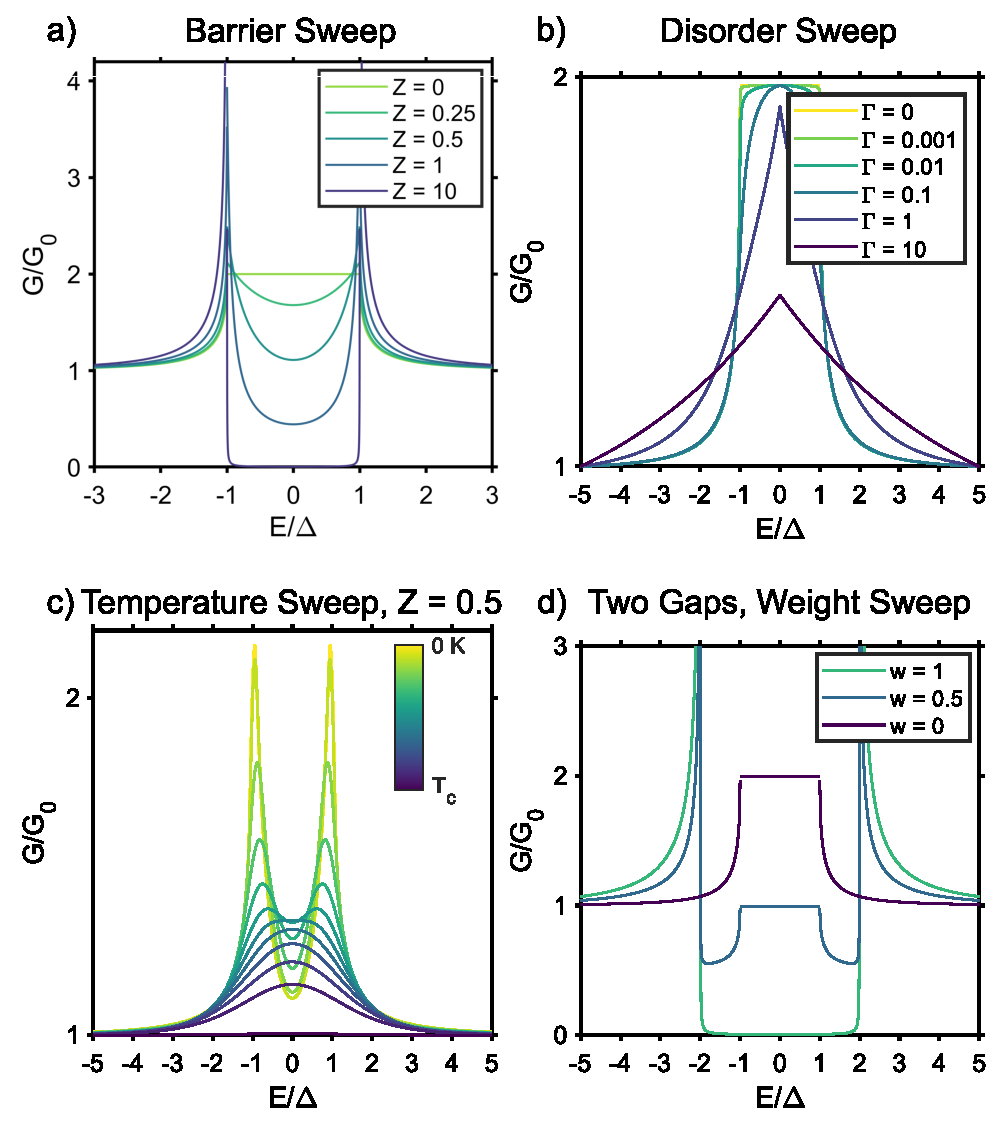
\includegraphics[width=\textwidth]{Appendices/Figures/BTKCalculations.eps}
    \caption{Various demonstrations of the differential conductance calculated using the algorithms described in A.2. a) Single gap, zero Kelvin sweep of the potential barrier strength $Z$. b) Single gap, zero Kelvin, zero barrier sweep of the thermal broadening parameter $\Gamma$. c) Single gap, half-strength barrier, temperature sweep. d) Two superconducting gaps where the second gap is twice as large as the first demonstrating the $w$ parameter in action.}
    \label{fig:BTKGraphs}
\end{figure}
\begin{algorithm}
\caption{Single Gap \ac{BTK} conductance}\label{zeroT}
\begin{algorithmic}[1]
\Function{BTK1g}{$meV, Z, \Delta_{SC}, \Gamma$}\Comment{Returns conductance vector.}
\State $N_{q}=\left|\frac{meV+i\Gamma}{\sqrt{(meV+i\Gamma)^{2}-\Delta_{SC}^{2}}}\right|$\Comment{quasi-particles \ac{DoS}}
\State $N_{p}=\frac{\Delta_{SC}}{\sqrt{(meV+i\Gamma)^{2}-\Delta_{SC}^{2}}} $\Comment{Pair \ac{DoS}}
\State $\tau_{n} = \frac{1}{1+Z^{2}}$\Comment{Define the transparency}
\State $\gamma = \frac{N_{q}-1}{N_{p}}$\Comment{Define $\gamma$ function. Not $\Gamma$!}
\State $G = \frac{1+\tau_{n}\left|\gamma\right|^{2}+\left(\tau_{n}-1\right)\left|\gamma^{2}\right|^{2}}{\left|1+\left(\tau_{n}-1\right)\gamma^{2}\right|^{2}}$\Comment{G will be a vector.}
\State \textbf{return} $G$, $\tau_{n}$\Comment{We return $\tau_{n}$ in preparation for the next function.}
\EndFunction
\end{algorithmic}
\end{algorithm}
This code is useful for understanding what the conductance looks like at various Z-values, Gap-sizes. The broadening term can be used (or fit) to simulate a finite temperature since (as the name suggests) it is basically a term that broadens the spectral peaks out.\par
If we want to incorporate the temperature in a more rigorous way we can take the outputs of the previous function then integrate the convolution of their product with the Fermi function (Algorithm 2).
\begin{algorithm}
\caption{BTK at finite temperature}
\begin{algorithmic}[1]
\State $G, \tau_{n} = BTK1g(meV, Z, \Delta_{SC}, \Gamma)$
\For{V in meV}
\State $f_{C} = G\tau_{n}\left(\frac{1}{e^{\left(e-V\right)/k_{b}T}}-\frac{1}{e^{E/k_{b}T+1}}\right)$\Comment{Convolution. Outputs a function.}
\State $I_{ns}(V) = \int_{-\infty}^{\infty}f_{C}dE$\Comment{Integrate function over all energies.}
\EndFor
\State $\frac{dI}{dV} = \left|\nabla(I_{NS})\right|$
\end{algorithmic}
\end{algorithm}
I've used an anonymous function since these codes were originally written in MatLab however the same task can be accomplished in Python with a lambda function instead. Alternatively, one could also skip the for-loop by implementing the numpy function numpy.convolve(vector1,vector2). Algorithm 3 is a simple extension that allows us to model the conductance with two superconducting gaps.\par
\begin{algorithm}
\caption{Two Gap BTK Fit}
\begin{algorithmic}[1]
\State $G_{1},\tau_{1} = BTK\_at\_finite\_temperature(meV,Z_{1},\Delta_{SC,1},\Gamma_{1})$
\State $G_{2},\tau_{2} = BTK\_at\_finite\_temperature(meV,Z_{2},\Delta_{SC,2},\Gamma_{2})$
\State $G = w*G_{1} + (w-1)*G_{2}$\Comment{$w$ ranges between 0 and 1.}
\end{algorithmic}
\end{algorithm}
Algorithm 4 is another simple function to either fit the temperature-dependence of the gaps to what's predicted via \ac{BCS} theory or use this function to generate a series of gap sizes for our \ac{BTK} versus temperature function later. I've presented this as a function so that it's easier to fit with, but this can be defined as an anonymous function (MatLab) or lambda function (Python) to reduce file complexity. 
\begin{algorithm}
\caption{BCS Gap}\label{euclid}
\begin{algorithmic}[1]
\Function{BCSGap}{$T$,$\Delta_{0},T_{c}$,$\alpha$}\Comment{SC gap at temperature T.}
\State $\Delta(T) = \left|1.74k_{b}T_{c}\left(1-\left(\frac{T}{T_{c}}\right)\right)^{\alpha}\right|$
\State \textbf{return} $\Delta(T)$
\EndFunction
\end{algorithmic}
\end{algorithm}
Finally Algorithm 5 denotes the whole script for modelling and plotting a range of temperatures to both single gap and two-gap BTK models using the above functions. Fitting the function varies by platform a bit but the pseudo-code is to define the ``BTK and finite temperature" file as the model as use the built-in fit functions.
\begin{algorithm}
\caption{BTK Temperature Fit}{BTKTempFit}
\begin{algorithmic}[1]
\State $Temps, dataCell = loadData(folder)$\Comment{``load\_data" is a script written by G. Osterhoudt.}
\State $fig = figure(1)$\Comment{Can use plt.subplot in Python}
\State $G_{0} = zeros(length(Temps))$\Comment{Will populate with normalization.}
\State $j = 0$\Comment{Iteration variable}
\For{T in Temps}
\State $\Delta_{SC} = BCSGap(T,\Delta_{0},T_{c},\alpha)$
\State $G = BTK\_at\_finite\_temperature(meV, Z, \Delta_{SC}, \Gamma)$
\State $Smooth$
\State $G_{0}(j) = G(end)$
\State $j += 1$
\State $plot(meV, G/G_{0})$
\EndFor
\end{algorithmic}
\end{algorithm}